\section{Policy Gradient с переиспользованием сэмплов}\label{TRPOPPOsection}

\subsection{Проблема переиспользования сэмплов}

В Policy Gradient схеме нам всегда приходится работать в on-policy режиме: нам нужны роллауты, сгенерированные при помощи текущей политики с параметрами $\theta$, чтобы посчитать градиент в точке $\theta$ и сделать шаг оптимизации. После этого будут нужны уже сэмплы из новой стратегии, поэтому единственное, что мы можем сделать с уже собранными данными --- почистить оперативную память.

Понятно, что это полное безобразие: допустим, агент долго вёл себя псевдослучайно и наконец наткнулся на какой-то хороший исход с существенным откликом среды. Схема сделает по ценному роллауту всего один градиентный шаг, что скорее всего не поможет модели выучить удачное поведение или значение отклика. После этого ценная информация никак не может быть использована и придётся дожидаться следующей удачи, что может случиться нескоро. Это очень sample inefficient и основная причина, почему от любого on-policy обучения в чистом виде нужно пытаться отойти. Полностью перейти в off-policy режим у нас не получится, но мы хотя бы научимся делать несколько градиентных шагов по одному собранному роллауту, и это даст свои плюшки.

Интуитивная идея дальнейшей теории в том, что мы хотим научиться считать градиент в точке текущих параметров, при этом используя сэмплы, полученные при помощи другой стратегии, возможно, недавней (очень похожей) версии той же стратегии. То, что стратегия сбора данных <<похожа>> на текущую, означает, что её траектории тоже в некотором смысле <<похожи>>: понятно, что это важно, ведь много информации о градиенте политики по около-оптимальным параметрам с траекторий случайного агента собрать не получится, просто потому что такие траектории у около-оптимальной стратегии почти не встретятся.

Итак, допустим мы хотим оптимизировать стратегию $\textcolor{ChadBlue}{\pi_\theta}$ по параметрам $\textcolor{ChadBlue}{\theta}$, используя только сэмплы из другой стратегии $\textcolor{ChadPurple}{\pi^{\old}}$ (в итоговой схеме это будет недавняя версия стратегии). В принципе, мы можем сделать это напрямую через importance sampling:
$$
\nabla_{\theta} J(\textcolor{ChadBlue}{\theta}) = \E_{\Traj \sim \textcolor{ChadPurple}{\pi^{\old}}} \frac{\mathcal{P}(\Traj \mid \textcolor{ChadBlue}{\pi_{\theta}})}{\mathcal{P}(\Traj \mid \textcolor{ChadPurple}{\pi^{\old}})} \sum_{t \ge 0} \nabla_{\theta} \log \textcolor{ChadBlue}{\pi_{\theta}}(a_t \mid s_t) \textcolor{ChadBlue}{A^\pi}(s_t, a_t)
$$
Появившийся коэффициент в принципе вычислим, поскольку вероятности переходов (которые мы не знаем) сокращаются:
$$\frac{\mathcal{P}(\Traj \mid \textcolor{ChadBlue}{\pi_\theta})}{\mathcal{P}(\Traj \mid \textcolor{ChadPurple}{\pi^{\old}})} = \frac{\prod\limits_{t \ge 0} \textcolor{ChadBlue}{\pi_\theta}(a_t \mid s_t)}{\prod\limits_{t \ge 0} \textcolor{ChadPurple}{\pi^{\old}}(a_t \mid s_t)}$$
Но, конечно, этот коэффициент ужасен: он может быть экспоненциально большим или маленьким и скорее всего затухнет или взорвётся. Поколдовать тут особо не получится, поскольку скорее всего мини-батч любого разумного размера будет доминироваться одной парой $s_t, a_t$ с самым большим значением коэффициента, и никакой стабильной процедурой оптимизации тут не пахнет. Нужно подойти с другой стороны...

\subsection{Суррогатная функция}

Вместо этого предлагается вспомнить RPI:
\begin{theorem}
\,
\begin{equation}\label{RPIdecoupled}
J(\textcolor{ChadBlue}{\pi_{\theta}}) = J(\textcolor{ChadPurple}{\pi^{\old}}) + \frac{1}{1 - \gamma}\E_{s \sim \textcolor{ChadBlue}{d_{\pi_{\theta}}}(s)} \E_{a \sim \textcolor{ChadBlue}{\pi_{\theta}}(a \mid s)} \textcolor{ChadPurple}{A^{\pi^{\old}}}(s_t, a_t)
\end{equation}
\begin{proof}
Из RPI \eqref{RPI} следует, что для любых двух стратегий верно 
$$J(\textcolor{ChadBlue}{\pi_{\theta}}) = J(\textcolor{ChadPurple}{\pi^{\old}}) + \E_{\Traj \sim \textcolor{ChadBlue}{\pi_{\theta}}} \sum_{t \ge 0} \gamma^t \textcolor{ChadPurple}{A^{\pi^{\old}}}(s_t, a_t)$$
Для получения формулы достаточно переписать мат.ожидание по траекториям из $\textcolor{ChadBlue}{\pi_{\theta}}$ через state visitation distribution, подставив в теореме \ref{th:decoupling_stoch} в качестве $f(s, a) \HM= \textcolor{ChadPurple}{A^{\pi^{\old}}}(s, a)$.
\end{proof}
\end{theorem}

\begin{proposition}
$$\textcolor{ChadBlue}{\nabla_\theta} J(\textcolor{ChadBlue}{\pi_{\theta}}) = \textcolor{ChadBlue}{\nabla_\theta} \frac{1}{1 - \gamma}\E_{s \sim \textcolor{ChadBlue}{d_{\pi_{\theta}}}(s)} \E_{a \sim \textcolor{ChadBlue}{\pi_{\theta}}(a \mid s)} \textcolor{ChadPurple}{A^{\pi^{\old}}}(s_t, a_t)$$
\end{proposition}

Окей, в формуле справа мы возьмём значение $\textcolor{ChadPurple}{A^{\pi^{\old}}}(s_t, a_t)$ из критика, которого мы можем обучать по сэмплам из $\textcolor{ChadPurple}{\pi^{\old}}$; мы также можем справиться с мат.ожиданием $\E_{a \sim \textcolor{ChadBlue}{\pi_{\theta}}(a \mid s)}$ при помощи importance sampling:

\begin{proposition}
\begin{equation}\label{perfectsurrogate}
\textcolor{ChadBlue}{\nabla_\theta} J(\textcolor{ChadBlue}{\pi_{\theta}}) = \textcolor{ChadBlue}{\nabla_\theta} \frac{1}{1 - \gamma} \E_{s \sim \textcolor{ChadBlue}{d_{\pi_{\theta}}}(s)} \E_{a \sim \textcolor{ChadPurple}{\pi^{\old}}(a \mid s)} \frac{\textcolor{ChadBlue}{\pi_{\theta}}(a \mid s)}{\textcolor{ChadPurple}{\pi^{\old}}(a \mid s)} \textcolor{ChadPurple}{A^{\pi^{\old}}}(s_t, a_t)
\end{equation}
\end{proposition}

В отличие от прошлой попытки применить importance sampling, здесь коэффициент --- это одно отношение, а не произведение большого числа отношений, поэтому он уже как-то терпим. Осталась последняя проблема: $\textcolor{ChadBlue}{d_{\pi_{\theta}}}(s)$. В роллаутах, сгенерированных при помощи $\textcolor{ChadPurple}{\pi^{\old}}$, состояния всё-таки будут приходить\footnote{с учётом забивания на $\gamma^t$ и наших прочих оговорок.} из $\textcolor{ChadPurple}{d_{\pi^{\old}}}(s)$, и тут мы importance sampling не сделаем даже при большом желании, так как просто не можем внятно оценить эти величины.

Рассмотрим аппроксимацию: что, если мы в формуле \eqref{perfectsurrogate} заменим $\textcolor{ChadBlue}{d_{\pi_{\theta}}}(s)$ на $\textcolor{ChadPurple}{d_{\pi^{\old}}}(s)$? Это, вообще говоря, будет какая-то другая функция.

\begin{definition}
Введём суррогатную функцию:
\begin{equation}\label{surrogate}
L_{\textcolor{ChadPurple}{\pi^{\old}}}(\textcolor{ChadBlue}{\theta}) \coloneqq \frac{1}{1 - \gamma}\E_{s \sim \textcolor{ChadPurple}{d_{\pi^{\old}}}(s)} \E_{a \sim \textcolor{ChadPurple}{\pi^{\old}}(a \mid s)} \frac{\textcolor{ChadBlue}{\pi_\theta}(a \mid s)}{\textcolor{ChadPurple}{\pi^{\old}}(a \mid s)} \textcolor{ChadPurple}{A^{\pi^{\old}}}(s, a)   
\end{equation}
\end{definition}

\begin{proposition}
Сэмплы из мат.ожиданий в суррогатной функции --- это сэмплы из роллаутов, сгенерированных при помощи $\textcolor{ChadPurple}{\pi^{\old}}$:
\begin{equation*}
L_{\textcolor{ChadPurple}{\pi^{\old}}}(\textcolor{ChadBlue}{\theta}) = \E_{\Traj \sim \textcolor{ChadPurple}{\pi^{\old}}} \sum_{t \ge 0} \gamma^t \frac{\textcolor{ChadBlue}{\pi_\theta}(a \mid s)}{\textcolor{ChadPurple}{\pi^{\old}}(a \mid s)} \textcolor{ChadPurple}{A^{\pi^{\old}}}(s, a)
\end{equation*}
\begin{proof}[Пояснение]
Применить теорему \ref{th:decoupling_stoch} в обратную сторону для $f(s, a) \HM= \frac{\textcolor{ChadBlue}{\pi_\theta}(a \mid s)}{\textcolor{ChadPurple}{\pi^{\old}}(a \mid s)} \textcolor{ChadPurple}{A^{\pi^{\old}}}(s, a)$
\end{proof}
\end{proposition}

\subsection{Нижняя оценка}

Итак, у нас есть аппроксимация нашего оптимизируемого функционала через суррогатную функцию, с которой мы можем работать:
$$J(\textcolor{ChadBlue}{\pi}) \approx J(\textcolor{ChadPurple}{\pi^{\old}}) + L_{\textcolor{ChadPurple}{\pi^{\old}}}(\textcolor{ChadBlue}{\theta}) = J(\textcolor{ChadPurple}{\pi^{\old}}) + \frac{1}{1 - \gamma}\E_{s \sim \textcolor{ChadPurple}{d_{\pi^{\old}}}(s)} \E_{a \sim \textcolor{ChadPurple}{\pi^{\old}}(a \mid s)} \frac{\textcolor{ChadBlue}{\pi_\theta}(a \mid s)}{\textcolor{ChadPurple}{\pi^{\old}}(a \mid s)} \textcolor{ChadPurple}{A^{\pi^{\old}}}(s, a)$$

Насколько эта аппроксимация хороша? Наша интуиция была в том, что если $\textcolor{ChadBlue}{\pi}$ <<похожа>> на $\textcolor{ChadPurple}{\pi^{\old}}$, то частоты посещения состояний у них тоже наверняка будут похожи. Формализовать <<похожесть>> стратегий можно, например, так:
\begin{definition}
Введём расстояние между стратегиями $\textcolor{ChadBlue}{\pi}$, $\textcolor{ChadPurple}{\pi^{\old}}$ как максимальную KL-дивергенцию между ними по всем состояниям:
$$\KL^{\max}(\textcolor{ChadPurple}{\pi^{\old}}, \textcolor{ChadBlue}{\pi}) \coloneqq \max_s \KL(\textcolor{ChadPurple}{\pi^{\old}}(a \mid s) \parallel \textcolor{ChadBlue}{\pi_\theta}(a \mid s))$$
\end{definition}

\begin{theoremBox}[label=th:Lapproximationestimation]{}
\,
\begin{equation*} 
\left| J(\textcolor{ChadBlue}{\pi_\theta}) - J(\textcolor{ChadPurple}{\pi^{\old}}) - L_{\textcolor{ChadPurple}{\pi^{\old}}}(\textcolor{ChadBlue}{\theta}) \right| \le C \KL^{\max}(\textcolor{ChadPurple}{\pi^{\old}}, \textcolor{ChadBlue}{\pi_{\theta}})
\end{equation*}
где $C$ --- константа, равная $C \HM= \frac{4 \gamma}{(1 - \gamma)^2} \max\limits_{s, a} |\textcolor{ChadPurple}{A^{\pi^{\old}}}(s, a)|$
\begin{proof}[Без доказательства; интересующиеся могут обратиться к \href{https://arxiv.org/abs/1502.05477}{статье по TRPO}...]
\end{proof}
\end{theoremBox}

Конечно, это очень грубая оценка, хотя бы потому, что она верна для произвольных MDP и произвольных двух стратегий. Но ключевой момент в том, что мы теперь формально можем вывести \emph{нижнюю оценку} (lower bound) на оптимизируемый функционал:
\begin{theorem}
\begin{equation}\label{lowerbound}
J(\textcolor{ChadBlue}{\pi_\theta}) - J(\textcolor{ChadPurple}{\pi^{\old}}) \ge L_{\textcolor{ChadPurple}{\pi^{\old}}}(\textcolor{ChadBlue}{\theta}) - C \KL^{\max}(\textcolor{ChadPurple}{\pi^{\old}}, \textcolor{ChadBlue}{\pi_{\theta}})
\end{equation}
\end{theorem}

\subsection{Оптимизация нижней оценки}

Возникает любопытнейшая идея:
\begin{theorem}
Процедура оптимизации
\begin{equation}\label{lowerboundopt}
\textcolor{ChadBlue}{\theta_{k+1}} \coloneqq \argmax_{\textcolor{ChadBlue}{\theta}} \left[ L_{\textcolor{ChadPurple}{\pi_{\theta_k}}}(\textcolor{ChadBlue}{\theta}) - C \KL^{\max}(\textcolor{ChadPurple}{\pi_{\theta_k}} \parallel \textcolor{ChadBlue}{\pi_\theta}) \right]
\end{equation}
гарантирует монотонное неубывание функционала: $J(\textcolor{ChadBlue}{\pi_{\theta_{k+1}}}) \ge J(\textcolor{ChadPurple}{\pi_{\theta_{k}}})$
\begin{proof}
В точке $\theta \HM= \theta_k$ суррогатная функция $L_{\pi_{\theta_k}}(\theta)$ равна нулю, поскольку
\begin{align*}
L_{\pi_{\theta_k}}(\theta_k) &= \\
= \{\text{по определению \eqref{surrogate}}\} &= \frac{1}{1 - \gamma}\E_{s \sim d_{\pi_{\theta_{k}}}(s)} \E_{a \sim \pi_{\theta_{k}}(a \mid s)} \frac{\pi_{\theta_{k}}(a \mid s)}{\pi_{\theta_{k}}(a \mid s)} A^{\pi_{\theta_{k}}}(s, a) = \\ 
&= \frac{1}{1 - \gamma}\E_{s \sim d_{\pi_{\theta_{k}}}(s)} \E_{a \sim \pi_{\theta_{k}}(a \mid s)} A^{\pi_{\theta_{k}}}(s, a) = \\
\{\text{следствие RPI \eqref{RPIdecoupled}}\} &= J(\pi_{\theta_{k}}) - J(\pi_{\theta_{k}}) = 0
\end{align*}

Понятно, что $\KL^{\max}(\pi_{\theta_k} \parallel \pi_\theta)$ в точке $\theta \HM= \theta_k$ тоже равна 0, так как во всех состояниях $\KL$ между одинаковыми стратегиями равна нулю. Значит, максимум нижней оценки не меньше нуля, а она есть нижняя оценка на $J(\textcolor{ChadBlue}{\pi_{\theta_{k+1}}}) -\HM J(\textcolor{ChadPurple}{\pi_{\theta_{k}}})$.
\end{proof}
\end{theorem}

\needspace{7\baselineskip}
\begin{wrapfigure}{r}{0.5\textwidth}
\vspace{-0.5cm}
\centering
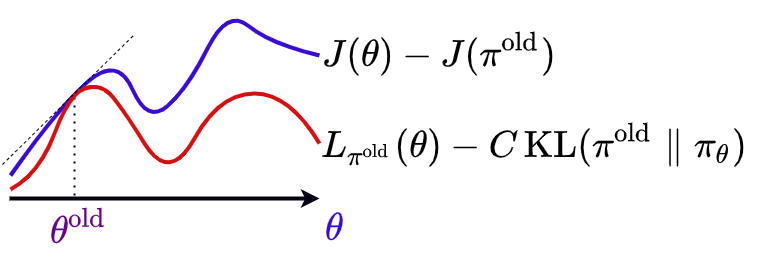
\includegraphics[width=0.5\textwidth]{Images/MM.png}
\vspace{-0.9cm}
\end{wrapfigure}

Итак, мы занимаемся типичным \emph{minorization-maximization} алгоритмом. Сначала мы подтягиваем нашу нижнюю оценку так, чтобы в текущей точке $\theta \HM= \theta^{\old}$ она в точности совпадала с оптимизируемой функцией (minorization). Затем мы начинаем при фиксированном $\textcolor{ChadPurple}{\theta^{\old}}$ оптимизировать по $\textcolor{ChadBlue}{\theta}$ не наш функционал (который мы не сможем оптимизировать без новых сэмплов из новой стратегии $\textcolor{ChadBlue}{\pi_\theta}$ с текущими значениями параметров), а нижнюю оценку, с которой умеем работать (maximization). 

Что мы получили процедуру, гарантирующую улучшение стратегии, звучит слишком хорошо! Где-то есть подвох... Что отделяет нас от такого теоретического алгоритма на практике? Ну, во-первых, наш критик $\textcolor{ChadPurple}{A^{\pi^{\old}}}$ неидеален и его оценка через сеть-критик будет смещённой, поэтому все теоретические гарантии уже на этом месте улетают в ближайшее окно. Постараемся об этом не думать.

Проблемы на этом не заканчиваются: мы не умеем ни считать константу $C$ (там есть максимум Advantage-функции по всем парам состояние-действие\footnote{мы могли бы оценить его сверху как $2R^{\max}$, где $R^{\max}$ --- максимальная награда, но это было бы непрактично грубой оценкой.}...), ни меру схожести стратегий $\KL^{\max}$. Последнее порешаем так: тихонько заменим максимум на среднее по состояниям:
$$\max_s \KL(\textcolor{ChadPurple}{\pi^{\old}}(a \mid s) \parallel \textcolor{ChadBlue}{\pi_\theta}(a \mid s)) \approx \E_{s \sim \textcolor{ChadPurple}{d_{\pi^{\old}}}(s)} \KL(\textcolor{ChadPurple}{\pi^{\old}}(a \mid s) \parallel \textcolor{ChadBlue}{\pi_\theta}(a \mid s))$$

Среднее берём по состояним из $\textcolor{ChadPurple}{d_{\pi^{\old}}}(s)$ исключительно из удобства, так как именно из него будут приходить состояния в роллаутах, сгенерированных $\textcolor{ChadPurple}{\pi^{\old}}$. Везде далее будем для сокращения использовать такую запись:
$$\KL(\textcolor{ChadPurple}{\pi^{\old}} \parallel \textcolor{ChadBlue}{\pi_\theta}) \coloneqq \E_{s \sim \textcolor{ChadPurple}{d_{\pi^{\old}}}(s)} \KL(\textcolor{ChadPurple}{\pi^{\old}}(a \mid s) \parallel \textcolor{ChadBlue}{\pi_\theta}(a \mid s))$$ 

Получаем такую задачу оптимизации:

\begin{equation}\label{lowerboundmean}
L_{\textcolor{ChadPurple}{\pi^{\old}}}(\textcolor{ChadBlue}{\theta}) - C \KL(\textcolor{ChadPurple}{\pi^{\old}} \parallel \textcolor{ChadBlue}{\pi_\theta}) \to \max_{\textcolor{ChadBlue}{\theta}}
\end{equation}

То есть, что мы получили: мы <<можем>> оптимизировать не $J(\textcolor{ChadBlue}{\pi_\theta}) - J(\textcolor{ChadPurple}{\pi^{\old}})$ по формуле \eqref{perfectsurrogate}, а нашу суррогатную функцию $L_{\textcolor{ChadPurple}{\pi^{\old}}}(\textcolor{ChadBlue}{\theta})$, но добавив штраф --- регуляризатор --- за различие между $\textcolor{ChadBlue}{\pi_\theta}$ и стратегией, из которой приходят данные $\textcolor{ChadPurple}{\pi^{\old}}$.

Однако, всё ещё осталась беда с константой $C$. Чтобы в очередной раз не потерять теоретические гарантии, она должна быть достаточно большой, чтобы превосходить константу из теоремы \ref{th:Lapproximationestimation}. Вообще, скорее всего, даже если бы мы знали эту константу, она была бы колоссальной (чего стоит только $(1 \HM- \gamma)^2$ в знаменателе) и практической пользы от такой нижней оценки всё равно много бы не было.

\subsection{Trust Region Policy Optimization (TRPO)}

В TRPO предлагается следующая интуиция. Когда мы делаем шаг градиентного спуска, мы рискуем сделать слишком длинный шаг, даже если он делается в верном направлении. При этом если лёрнинг рейт выбрать маленьким во избежание подобной ситуации, модель будет обучаться очень долго (а у нас тут сэмплы на каждый шаг сжигаются!). Авторам хочется делать какой-нибудь лайн-сёрч и использовать методы второго порядка для обучения параметров стратегии, но с основной целью запретить опасно большие изменения стратегии на одном шаге.

\begin{wrapfigure}{r}{0.2\textwidth}
\vspace{-0.5cm}
\centering
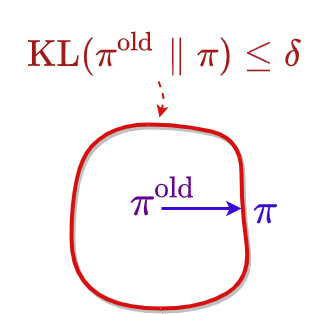
\includegraphics[width=0.2\textwidth]{Images/HardTrustRegion.png}
\vspace{-0.9cm}
\end{wrapfigure}

Основная идея заключается в переходе от оптимизации \eqref{lowerboundmean} без ограничений к задаче оптимизации с ограничением в <<\emph{trust region}>> форме:
\begin{equation}\label{trustregion}
\begin{cases}
L_{\textcolor{ChadPurple}{\pi^{\old}}}(\textcolor{ChadBlue}{\theta}) \to \max\limits_{\textcolor{ChadBlue}{\theta}} \\
\KL(\textcolor{ChadPurple}{\pi^{\old}} \parallel \textcolor{ChadBlue}{\pi_\theta}) \le \delta
\end{cases}
\end{equation}

Мол, наше второе слагаемое как раз есть штраф за очень большой шаг (да ещё и с какой-то очень большой, плюс и неизвестной нам константой $C$), поэтому давайте оптимизировать суррогатную функцию $L_{\textcolor{ChadPurple}{\pi^{\old}}}(\textcolor{ChadBlue}{\theta})$ с жёстким ограничением на длину шага.

Вообще говоря, мы получили задачу для оптимизации $L_{\textcolor{ChadPurple}{\pi^{\old}}}(\textcolor{ChadBlue}{\theta})$ методом \emph{натуральных градиентов} (natural gradient): мы оптимизируем функцию, разрешая не шаг некоторой длины по градиенту в пространстве параметров, а шаг некоторой длины в пространстве параметрически заданных распределений. Подробнее о натуральном градиенте можно прочитать в приложении \ref{appendix:ng}. Если раньше градиентный шаг мог сильно поменять стратегию (как распределение в пространстве действий), при том что для других небольших изменений распределения было бы необходимо сильно менять параметры $\textcolor{ChadBlue}{\theta}$, то здесь $\delta$ ограничивает изменение самой стратегии в терминах $\KL$-дивергенции. Ограничение $\delta$ нам при этом всё равно нужно будет выбрать, это аналог лёрнинг-рейта в <<trust region формах>> методов оптимизации.

Как будем задачу \ref{trustregion} решать? В контексте нашей задачи мы собрали при помощи текущей стратегии некоторое количество данных для Монте-Карло оценок всех мат.ожиданий (в этот момент $\pi^{\old} \HM= \pi_\theta$) и хотим решить задачу \ref{trustregion}, зафиксировав $\textcolor{ChadPurple}{\pi^{\old}}$ и оптимизируя параметры $\textcolor{ChadBlue}{\theta}$. Обозначим параметры $\textcolor{ChadPurple}{\pi^{\old}}$ как $\textcolor{ChadPurple}{\theta^{\old}}$. Аппроксимируем оптимизируемый функционал $L_{\textcolor{ChadPurple}{\pi^{\old}}}(\textcolor{ChadBlue}{\theta})$ разложением Тейлора до первого порядка с центром в точке $\theta = \theta^{\old}$, а ограничение --- до второго. До второго --- потому что слагаемое первого порядка ноль.

\begin{proposition}
В точке $\theta = \theta^{\old}$ первый член разложения ограничения в ряд Тейлора равен нулю:
\begin{equation*}
\forall s \colon \left. \textcolor{ChadBlue}{\nabla_\theta} \KL(\textcolor{ChadPurple}{\pi^{\old}} \parallel \textcolor{ChadBlue}{\pi_\theta}) \right|_{\theta = \theta^{\old}} = 0
\end{equation*}
\begin{proof}
$\KL$-дивергенция в этой точке равна 0 как среднее по состояниям дивергенций между одинаковыми распределениями, следовательно как функция от $\textcolor{ChadBlue}{\theta}$ она достигает в этой точке глобального минимума $\Rightarrow$ градиент равен нулю.
\end{proof}
% \begin{proof}[Доказательство непосредственной проверкой]
% $$\left. \textcolor{ChadBlue}{\nabla_\theta} \KL(\textcolor{ChadPurple}{\pi^{\old}} \parallel \pi_\theta) \right|_{\theta = \theta^{\old}} = \left. \E_{\textcolor{ChadPurple}{\pi^{\old}}(a \mid s)} \textcolor{ChadBlue}{\nabla_\theta} \log \pi_\theta(a \mid s) \right|_{\theta = \theta^{\old}} = \E_{\pi_{\theta^{\old}}} \textcolor{ChadBlue}{\nabla_\theta} \log \pi_{\theta^{\old}}(a \mid s) = 0$$
% \end{proof}
\end{proposition}

Итак, введём обозначения для предложенного разложения. Пусть $g$ --- градиент $L_{\textcolor{ChadPurple}{\pi^{\old}}}(\textcolor{ChadBlue}{\theta})$ по параметрам $\textcolor{ChadBlue}{\theta}$ в точке $\theta = \theta^{\old}$, а $F$ --- гессиан ограничения в точке $\theta = \theta^{\old}$:
\begin{equation}\label{trpo_gradient}
    g := \left. \textcolor{ChadBlue}{\nabla_\theta} L_{\textcolor{ChadPurple}{\pi^{\old}}}(\textcolor{ChadBlue}{\theta}) \right|_{\theta = \theta^{\old}}
\end{equation}
\begin{equation}\label{trpo_hessian}
    F := \left. \textcolor{ChadBlue}{\nabla^2_\theta} \KL(\textcolor{ChadPurple}{\pi^{\old}} \parallel \textcolor{ChadBlue}{\pi_\theta}) \right|_{\theta = \theta^{\old}}
\end{equation}

В этих обозначениях аппроксимация задачи получается следующая:
\begin{equation}\label{approximatetrustregion}
\begin{cases}
\langle g , \textcolor{ChadBlue}{\theta} - \textcolor{ChadPurple}{\theta^{\old}} \rangle \to \max\limits_{\textcolor{ChadBlue}{\theta}} \\
\frac{1}{2} (\textcolor{ChadBlue}{\theta} - \textcolor{ChadPurple}{\theta^{\old}})^T F (\textcolor{ChadBlue}{\theta} - \textcolor{ChadPurple}{\theta^{\old}}) \le \delta
\end{cases}
\end{equation}

Градиент $g$, на самом деле, весьма любопытен:
\begin{proposition}
Градиент $g$ совпадает с градиентом из алгоритма Advantage Actor Critic \eqref{advantagepg}.
\begin{proof}
\begin{align*}g = \left. \textcolor{ChadBlue}{\nabla_\theta} L_{\textcolor{ChadPurple}{\pi^{\old}}}(\textcolor{ChadBlue}{\theta}) \right|_{\theta = \theta^{\old}} &= \frac{1}{1 - \gamma}\E_{s \sim \textcolor{ChadPurple}{d_{\pi^{\old}}}(s)} \E_{a \sim \textcolor{ChadPurple}{\pi^{\old}}(a \mid s)} \frac{\left. \textcolor{ChadBlue}{\nabla_\theta} \textcolor{ChadBlue}{\pi_\theta}(a \mid s) \right|_{\theta = \theta^{\old}}}{\textcolor{ChadPurple}{\pi^{\old}}(a \mid s)} \textcolor{ChadPurple}{A^{\pi^{\old}}}(s, a) = \\
= \{ \substack{\text{замечаем определение} \\ \text{производной логарифма} }\} &= \frac{1}{1 - \gamma}\E_{s \sim \textcolor{ChadPurple}{d_{\pi^{\old}}}(s)} \E_{a \sim \textcolor{ChadPurple}{\pi^{\old}}(a \mid s)} \left. \textcolor{ChadBlue}{\nabla_\theta} \log \textcolor{ChadBlue}{\pi_\theta}(a \mid s) \right|_{\theta = \theta^{\old}} \textcolor{ChadPurple}{A^{\pi^{\old}}}(s, a)
\end{align*}
что в точности есть градиент обычного ActorCritic c бэйзлайном в точке $\theta = \theta^{\old}$.
\end{proof}
\end{proposition}

\begin{theorem}
Решение аппроксимированной задачи \eqref{approximatetrustregion} есть
$$\theta - \theta^{\old} = kF^{-1}g$$
где скалярный коэффициент пропорциональности $k$ можно посчитать по формуле $k = \sqrt{\frac{2 \delta}{g^TF^{-1}g}}$
\begin{proof}
Составляем лагранжиан (условие входит с минусом, т.к. максимум поменяем на минимум):
$$\mathcal{L}(\lambda, \theta) = -g^T(\theta - \theta^{\old}) + \lambda \left( \frac{1}{2} (\theta - \theta^{\old})^T F (\theta - \theta^{\old}) - \delta \right)$$
Дифференцируем лагранжиан и приравниваем к нулю:
$$\nabla_\theta \mathcal{L}(\lambda, \theta) = -g + \lambda F (\theta - \theta^{\old}) = 0$$
Отсюда получаем:
\begin{equation}\label{solvetrustregion}
\theta - \theta^{\old} = \frac{1}{\lambda} F^{-1}g
\end{equation}
Осталось найти значение $\lambda$. Поскольку решение должно быть допустимой точкой, а оптимизируемый функционал линеен, понятно, что ограничение из задачи превратится в равенство и будет достигнуто на границе. То есть:
$$\frac{1}{2} (\theta - \theta^{\old})^T F (\theta - \theta^{\old}) = \delta$$
Подставляем найденное решение \eqref{solvetrustregion}:
$$\frac{1}{2} \left( \frac{1}{\lambda} F^{-1}g \right)^T F \left( \frac{1}{\lambda} F^{-1}g \right) = \frac{1}{2 \lambda^2} g^TF^{-1}g = \delta$$
Отсюда находим коэффициент\footnote{однозначно в силу положительности коэф. Лагранжа; число $g^TF^{-1}g$ положительно в силу того, что гессиан KL-дивергенции является матрицей Фишера и поэтому является положительно определённой матрицей (см. приложение \ref{appendix:fishermatrix}). Естественно, усреднение по состояниям не нарушает этого факта.}):
$$\lambda = \sqrt{\frac{g^TF^{-1}g}{2 \delta}}$$
Обратная дробь $\frac{1}{\lambda}$, соответственно, является коэффициентом пропорциональности.
\end{proof}
\end{theorem}

Итак, что мы делаем на практике. Во-первых, собираем большой-большой роллаут (порядка 1024 транзишнов суммарно по средам), чтобы возможно было хоть сколько-то адекватно оценивать гессиан $F$ \eqref{trpo_hessian}. Затем, считаем градиент $g$ \eqref{trpo_gradient} аналогично Actor-Critic методу. Далее мы хотим решить систему линейных уравнений:
$$F \left(\theta - \theta^{\old}\right) = g$$
Хранить в памяти гессиан и тем более обращать для нейросеток мы, конечно, не будем и воспользуемся \emph{методом сопряжённых градиентов} (conjugate gradient method)\footnote{прочитать про него можно, например, \href{https://ru.wikipedia.org/wiki/Метод_сопряжённых_градиентов_(для_решения_СЛАУ)}{в википедии}}, который позволяет решать систему линейных уравнений итеративно, на каждой итерации требуя лишь вычислять $Fh$ для некоторых векторов $h$. Нам придётся для каждой итерации метода сопряжённых градиентов сделать два обратных прохода по вычислительному графу (дважды вычислять все производные: сначала по функции, для которой мы хотим посчитать гессиан, чтобы получить градиент $f$, затем для градиента функции $\langle f, h \rangle$), но до сходимости сводить алгоритм не будем и остановим после порядка 10 итераций. Процедура получается дороговатой всё равно, но поскольку в деле замешан гессиан, то что поделать --- мы практически выходим в методы оптимизации второго порядка.

Посчитали приближение $F^{-1}g$, дальше возникает проблема: нам нужно домножить вектор на коэффициент $k$, который напрямую зависит от $\delta$. Мы могли бы поставить $\delta$ гиперпараметром как лёрнинг рейт в обычном градиентном спуске, но всё-таки мы боремся за то, чтобы делать шаги <<правильного>> размера. Мы уже знаем направление $F^{-1}g$, в котором будем менять параметры политики, но не знаем, насколько.

Предлагается устроить \emph{line-search} по аналогии с методами оптимизации, а то есть процедуру бэктрэкинга. Выставляем какое-нибудь большое значение $\delta$ (это начальное значение --- гиперпараметр) и считаем коэффициент пропорциональности $k = \sqrt{\frac{2 \delta}{g^TF^{-1}g}}$ (заметим, что $F^{-1}g$ приближённо мы уже посчитали в методе сопряжённых градиентов). Дальше авторы предлагают проверить, а правда ли наше мы остались внутри trust region-а, то есть соблюли условие $\KL(\textcolor{ChadPurple}{\pi^{\old}} \parallel \textcolor{ChadBlue}{\pi_\theta}) \HM\le \delta$. Мы могли нарушить это условие как из-за перехода к приближённой задаче \eqref{approximatetrustregion}, так и из-за приближённого её решения через метод сопряжённых градиентов; если таки нарушили, то уменьшаем $\delta$ в, допустим, два раза и перепроверяем.

Мы уже шагнули на границу нашего региона доверия, максимально отступив от $\textcolor{ChadPurple}{\pi^{\old}}$, использовавшихся для сбора данных. Соответственно, смысла <<продолжать>> оптимизировать нижнюю оценку дальше, разложив функционал в $\textcolor{ChadBlue}{\theta} \ne \textcolor{ChadPurple}{\theta^{\old}}$, нет; нужно перестраивать нижнюю оценку, то есть собирать новые данные при помощи обновлённой стратегии. То есть переиспользовать данные мы не научились, но мы научились делать тяжёлые и дорогие, но хорошие шаги оптимизации. 

\vspace{0.4cm}
\begin{center}
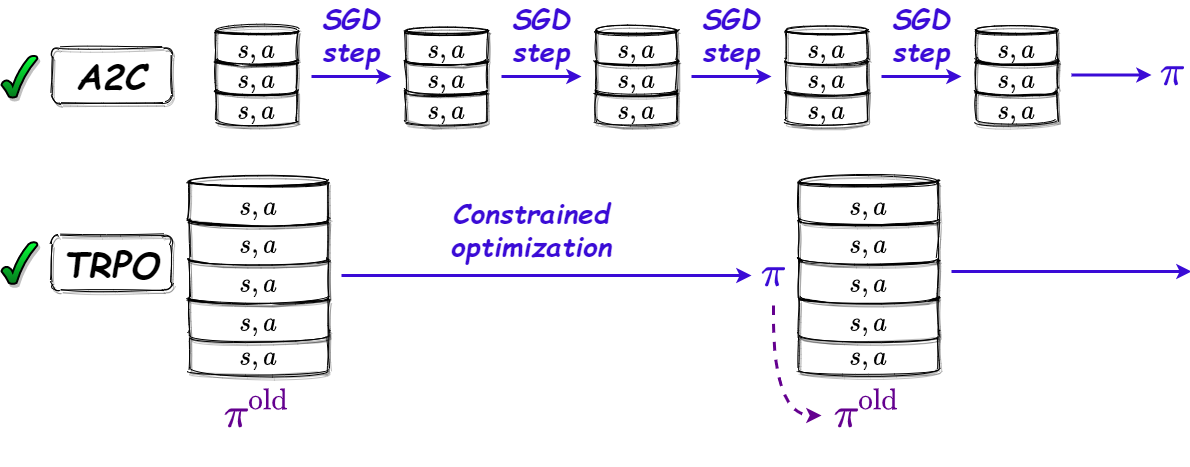
\includegraphics[width=0.9\textwidth]{Images/TRPOpipeline2.png}
\end{center}

\begin{remark}
В текущем виде в TRPO критика всё ещё нужно оптимизировать также, как в A2C, то есть собирая маленькие роллауты и делая небольшие шаги. Не очень удобно делать это параллельно со сбором больших роллаутов для актёра, да и оптимизировать актёра и критика в этой схеме, получается, придётся раздельно (иметь для них две раздельные сетки). Поскольку роллауты собирают большие, в имплементациях на критика иногда вообще забивают и используют Монте-Карло оценку как в REINFORCE, просто доигрывая игры до конца (всё равно нам длинные роллауты нужны).
\end{remark}

\subsection{Proximal Policy Loss}

Proximal Policy Optimization (PPO) --- альтернативный способ рассуждения после вывода нижней оценки \eqref{lowerboundmean}. Давайте не будем прибегать к методам оптимизации, требующим какие-либо гессианы, и будем оптимизировать нижнюю оценку напрямую обычным градиентным спуском, где $C$ --- гиперпараметр:

\begin{equation}\label{lowerboundunconstrained}
\E_{s \sim \textcolor{ChadPurple}{d_{\pi^{\old}}}(s)} \E_{a \sim \textcolor{ChadPurple}{\pi^{\old}}(a \mid s)} \left[ \frac{\textcolor{ChadBlue}{\pi_\theta}(a \mid s)}{\textcolor{ChadPurple}{\pi^{\old}}(a \mid s)} \textcolor{ChadPurple}{A^{\pi^{\old}}}(s, a) - C \KL(\textcolor{ChadPurple}{\pi^{\old}} \parallel \textcolor{ChadBlue}{\pi_\theta}) \right] \to \max_{\textcolor{ChadBlue}{\theta}}
\end{equation}

Сделать так напрямую в лоб не получится; давайте поймём почему. Какого размера датасет нам понадобится для такого пайплайна? Собрать данных на мини-батч или несколько и <<воспользоваться ими несколько раз>> не получится: Монте-Карло оценки мат.ожиданий в наших функциях потерь просто будут скоррелированы. Чтобы по данным из $\textcolor{ChadPurple}{\pi^{\old}}$ прооптимизировать $\textcolor{ChadBlue}{\theta}$ несколькими шагами градиентного спуска, нужно, чтобы мини-батчи были достаточно разными. Это значит, что при помощи $\textcolor{ChadPurple}{\pi^{\old}}$ придётся собрать датасет достаточно большого размера.

\vspace{0.4cm}
\begin{center}
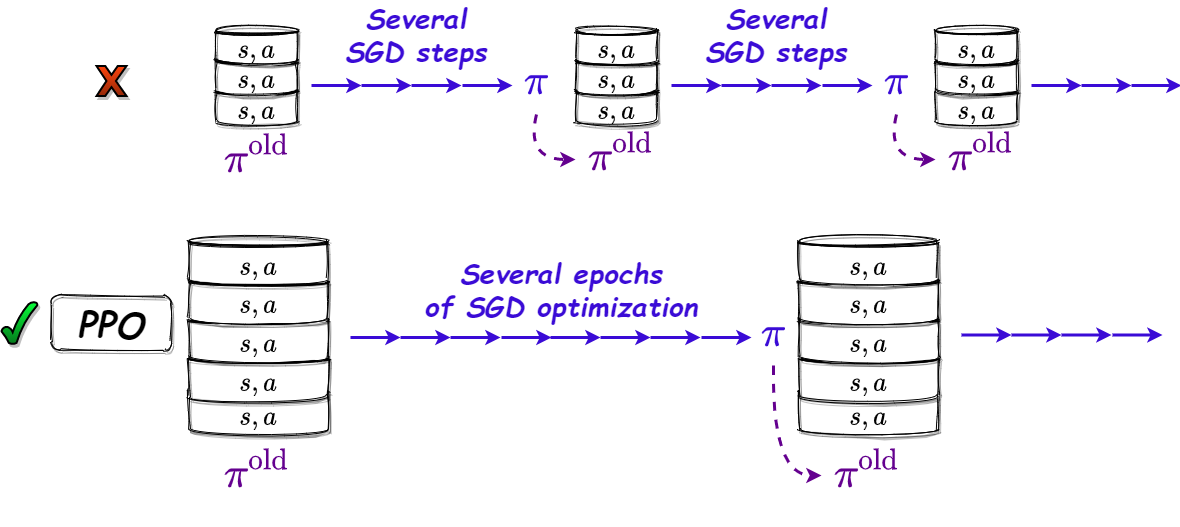
\includegraphics[width=0.9\textwidth]{Images/PPOpipeline2.png}
\end{center}

\begin{wrapfigure}{r}{0.3\textwidth}
\vspace{-0.5cm}
\centering
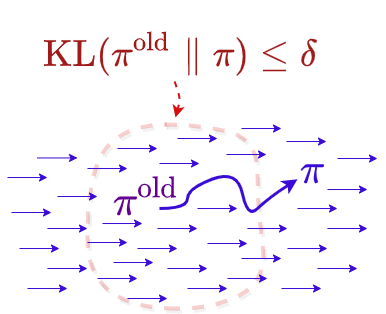
\includegraphics[width=0.3\textwidth]{Images/TrustRegion1.png}
\vspace{-0.5cm}
\end{wrapfigure}

Чтобы что-то выиграть от такого процесса, нужно пройтись по датасету несколькими эпохами (иначе тот же A2C был бы выгоднее за счёт свежести данных). Это значит, что шагов градиентной оптимизации понадобится сделать достаточно много. Это приводит к тому, что потенциально стратегия обновляется за время оптимизации на одном датасете относительно сильно: вместе с тем, что небольшое изменение в пространстве параметров может приводить к большому изменению стратегии $\pi$ (в пространстве распределений) без введения жёсткого региона доверия стратегия может начать сколь угодно сильно подстраиваться под те оценки критика, которые мы выдадим парам в датасете. На тех парах $s, a$, где оценка Advantage положительна (в том числе из-за Монте-Карло оценки Q-функции, которая в on-policy режиме принципиально содержит сэмплы награды из только что сыгранных шагов), стратегия начнёт улетать к вырожденной, а вероятности на парах $s, a$ с отрицательной оценкой Advantage начнут уплывать в ноль. В итоге начинают регулярно встречаться взрывающиеся или затухающие importance sampling коэффициенты $\frac{\textcolor{ChadBlue}{\pi_\theta}(a \mid s)}{\textcolor{ChadPurple}{\pi^{\old}}(a \mid s)}$, мини-батч становится несбалансированным и в плане <<весов>> объектов.

Предлагается полечить костылём: обрезать. Обозначим importance sampling коэффициент
$$\rho(\textcolor{ChadBlue}{\theta}) \coloneqq \frac{\textcolor{ChadBlue}{\pi_\theta}(a \mid s)}{\textcolor{ChadPurple}{\pi^{\old}}(a \mid s)}$$
и обрежем его как
$$\rho^{\clip}(\textcolor{ChadBlue}{\theta}) \coloneqq \clip(\rho(\textcolor{ChadBlue}{\theta}), 1 - \epsilon, 1 + \epsilon),$$
где $\epsilon \in (0, 1)$ --- гиперпараметр (типичный выбор --- 0.1 или 0.2). Рассмотрим альтернативную функцию потерь:
\begin{equation*}
\E_{s \sim \textcolor{ChadPurple}{d_{\pi^{\old}}}(s)} \E_{a \sim \textcolor{ChadPurple}{\pi^{\old}}(a \mid s)} \left[ \rho^{\clip}(\textcolor{ChadBlue}{\theta}) \textcolor{ChadPurple}{A^{\pi^{\old}}}(s, a) - C \KL(\textcolor{ChadPurple}{\pi^{\old}} \parallel \textcolor{ChadBlue}{\pi_\theta}) \right] \to \max_{\textcolor{ChadBlue}{\theta}}
\end{equation*}

\begin{wrapfigure}{r}{0.3\textwidth}
\vspace{-0.5cm}
\centering
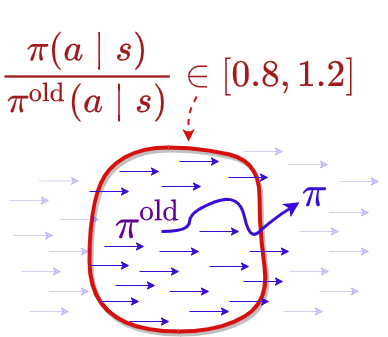
\includegraphics[width=0.3\textwidth]{Images/TrustRegion2.png}
\vspace{-0.5cm}
\end{wrapfigure}
Что случилось с градиентами при таком изменении? Если происходит обрезка, то есть если $\rho(\textcolor{ChadBlue}{\theta})$ не попадает в указанный диапазон $[1 - \epsilon, 1 + \epsilon]$, то градиент основного слагаемого, как легко видеть, зануляется. Иначе он остаётся без изменений:
$$\textcolor{ChadBlue}{\nabla_\theta} \rho^{\clip}(\textcolor{ChadBlue}{\theta}) = 
\begin{cases}
0 \quad &\rho(\textcolor{ChadBlue}{\theta}) \not\in [1 - \epsilon, 1 + \epsilon] \\
\textcolor{ChadBlue}{\nabla_\theta} \rho(\textcolor{ChadBlue}{\theta}) \quad &\rho(\textcolor{ChadBlue}{\theta}) \in [1 - \epsilon, 1 + \epsilon] \\
\end{cases}
$$
Таким образом, подобный клиппинг --- <<мягкий trust region>>: как только стратегия слишком отдаляется от $\textcolor{ChadPurple}{\pi^{\old}}$ на данной паре $s, a$, градиенты <<перестают>> обновлять эту пару. Это не означает, что стратегия в этой паре не продолжит меняться: с ней потенциально в градиентном спуске может происходить всё что угодно, она может продолжать изменяться за счёт <<схожих>> пар $s, a$, например, которые ещё остаются <<внутри trust region-а>> или, в конце концов, из-за моментума в алгоритме стохастической оптимизации\footnote{в RL, как и в глубоком обучении, обычный стохастический градиентный спуск не используется, а вместо этого используется, например, Adam.}.

Замена функции потерь лишила нас в очередной раз <<гарантий нижней оценки>>: хотелось бы, чтобы при достаточно большой константе $C$ эти гарантии оставались. Поэтому мы не просто заменим функцию потерь на версию с обрезкой, а возьмём минимум между ними: так мы сохраним свойство нижней оценки и гарантируем, что функционал \eqref{lowerboundunconstrained} не увеличился: 
\begin{equation}\label{PPOlowerbound}
\E_{s \sim \textcolor{ChadPurple}{d_{\pi^{\old}}}(s)} \E_{a \sim \textcolor{ChadPurple}{\pi^{\old}}(a \mid s)}  \left[ \min \left( \rho(\textcolor{ChadBlue}{\theta}) \textcolor{ChadPurple}{A^{\pi^{\old}}}(s, a), \rho^{\clip}(\textcolor{ChadBlue}{\theta}) \textcolor{ChadPurple}{A^{\pi^{\old}}}(s, a)\right) - C \KL(\textcolor{ChadPurple}{\pi^{\old}} \parallel \textcolor{ChadBlue}{\pi_\theta}) \right] \to \max_\theta
\end{equation}

Интуиция нижней оценки здесь, на самом деле, под очень большим вопросом. Авторы алгоритма на этом этапе в ablation studies внезапно обнаружили, что на слагаемое с $\KL$-дивергенцией можно внезапно забить (выставить $C \HM= 0$), и эмпирические результаты не изменятся. Обычно в имплементациях PPO $\KL$-дивергенции в функционале по дефолту нет, и итого оптимизируемый функционал выглядит просто вот так:
\begin{equation}\label{PPOobjective}
\E_{s \sim \textcolor{ChadPurple}{d_{\pi^{\old}}}(s)} \E_{a \sim \textcolor{ChadPurple}{\pi^{\old}}(a \mid s)} \min \left( \rho(\textcolor{ChadBlue}{\theta}) \textcolor{ChadPurple}{A^{\pi^{\old}}}(s, a), \rho^{\clip}(\textcolor{ChadBlue}{\theta}) \textcolor{ChadPurple}{A^{\pi^{\old}}}(s, a)\right) \to \max_\theta
\end{equation}

На этом месте гробик связи между алгоритмом и теорией засыпается землёй. Но что же произошло? Мы ввели обрезку (имеющую некоторый смысл trust region-а) и взятие минимума между двумя функциями потерь; если обрезка так хорошо <<смоделировала>> trust region, что регуляризатор (слагаемое с $\KL$-дивергенцией) и не нужен, то какой физический смысл имеет минимум? 

Итак, давайте поймём, какую роль в интуиции trust region-а играет взятие минимума, посмотрев на градиенты для одной пары $s, a$. Введение минимума всё ещё <<выкидывает>> из градиентов функционала пары $s, a$, на которых коэффициент $r(\theta)$ не близок к 1; или же оставляет градиент без изменений. Зануление градиента происходит в случае, если происходит сразу два события: минимум достигается на <<обрезанной>> версии градиента и importance sampling вес вышел за границы. Рассмотрим всевозможные случаи:

$$\textcolor{ChadBlue}{\nabla_\theta} \min \left( \rho(\textcolor{ChadBlue}{\theta}) \textcolor{ChadPurple}{A^{\pi^{\old}}}(s, a), \rho^{\clip}(\textcolor{ChadBlue}{\theta}) \textcolor{ChadPurple}{A^{\pi^{\old}}}(s, a)\right) = 
\begin{cases}
0 \quad & \rho(\textcolor{ChadBlue}{\theta}) > 1 + \epsilon, \textcolor{ChadPurple}{A^{\pi^{\old}}}(s, a) \ge 0 \\
\textcolor{ChadBlue}{\nabla_\theta} \rho(\textcolor{ChadBlue}{\theta}) \quad &\rho(\textcolor{ChadBlue}{\theta}) \le 1 + \epsilon, \textcolor{ChadPurple}{A^{\pi^{\old}}}(s, a) \ge 0 \\
0 \quad & \rho(\textcolor{ChadBlue}{\theta}) < 1 - \epsilon, \textcolor{ChadPurple}{A^{\pi^{\old}}}(s, a) < 0 \\
\textcolor{ChadBlue}{\nabla_\theta} \rho(\textcolor{ChadBlue}{\theta}) \quad &\rho(\textcolor{ChadBlue}{\theta}) \ge 1 - \epsilon, \textcolor{ChadPurple}{A^{\pi^{\old}}}(s, a) < 0 \\
\end{cases}
$$

\needspace{13\baselineskip}
\begin{wrapfigure}{r}{0.3\textwidth}
\vspace{-0.25cm}
\centering
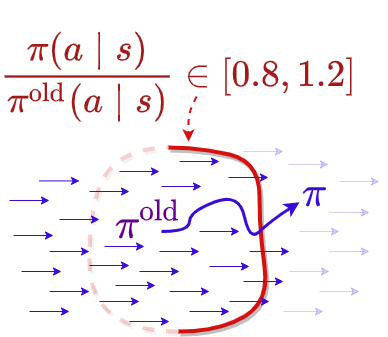
\includegraphics[width=0.3\textwidth]{Images/TrustRegion3.png}
\vspace{-0.25cm}
\end{wrapfigure}
Внимательно вглядевшись в эту <<таблицу>>, становится понятно, что происходит. Если оценка критика положительна, градиенты говорят увеличивать $\textcolor{ChadBlue}{\pi_\theta}(a \mid s)$; importance sampling вес повышается, и в какой-то момент случится обрезка по $1 + \epsilon$. Но если оценка критика положительна, и градиенты указывают увеличивать вероятность, а она по какой-то причине уменьшилась (такое вполне возможно в процессе оптимизации) и даже <<вылетела за границы trust region>>, то градиенты не зануляются: она вылетела <<не с той стороны>>! Симметричная ситуация случится при отрицательной оценке критика: вероятность должна уменьшаться, но сильно за счёт обрезки уменьшиться она не может, а за счёт оператора минимума при случайном увеличении градиенты продолжат тянуть вероятности <<к барьеру>>. Мы получили этакий <<полуоткрытый trust region>>.

\subsection{Clipped Value Loss}

\begin{wrapfigure}{r}{0.4\textwidth}
\vspace{-0.5cm}
\centering
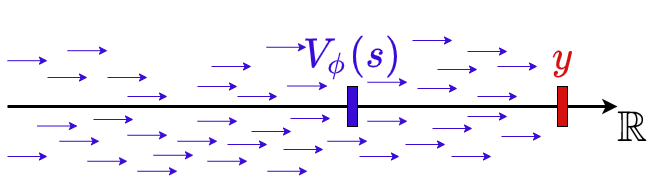
\includegraphics[width=0.4\textwidth]{Images/ValueTrustRegion1.png}
%\vspace{-0.5cm}
\end{wrapfigure}
Применим аналогичную идею <<полуоткрытого trust region-а>> для лосса критика. Пусть для данного состояния $s$ наша аппроксимация V-функции выдаёт $V^{\pi}_{\phi}(s)$, а таргет равен $y$. Обычно мы бы минимизировали MSE:
$$\Loss_1(\phi) \coloneqq (V^{\pi}_{\phi}(s) - y)^2$$

Однако, если таргет $y$ содержит в себе в том числе какие-то Монте-Карло оценки и переиспользуется <<несколько раз>> из небольшого датасета, то мы не хотим на него переобучаться. Пусть на момент сбора датасета критик выдавал для данного состояния $V^{\old}(s)$; таргет указывает лишь направление, в котором мы хотим изменить значение выхода критика, но, как и в любой стохастической аппроксимации, мы не хотим <<заменять жёстко>> выход $V^{\pi}_{\phi}(s)$ на $y$, а лишь сдвинуть в его сторону. Для этого добавим и вычтем в MSE $V^{\old}(s)$:
$$\Loss_1(\phi) = (V^{\pi}_{\phi}(s) - V^{\old}(s) - (y - V^{\old}(s)))^2$$

\begin{wrapfigure}{r}{0.4\textwidth}
%\vspace{-0.5cm}
\centering
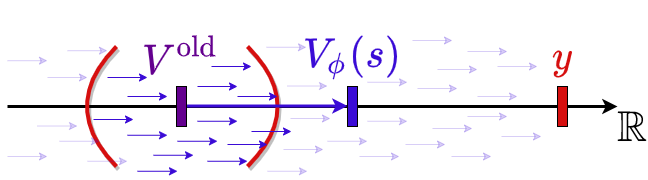
\includegraphics[width=0.4\textwidth]{Images/ValueTrustRegion2.png}
%\vspace{-0.5cm}
\end{wrapfigure}
Теперь мы сравниваем не выход сети с таргетом, а изменение значения выхода критика с <<желаемым изменением>> (на самом деле, просто оценкой Advantage; $y - V^{\old}(s)$ используется в качестве аппроксимации $\Psi(s, a)$). Введём другую функцию потерь, с <<обрезкой>>, которая построит <<мягкий trust-region>> и будет занулять градиенты, как только $V^{\pi}_{\phi}(s)$ станет непохожим на $V^{\old}(s)$:
$$\Loss_2(\phi) \coloneqq (\clip(V^{\pi}_{\phi}(s) - V^{\old}(s), \epsilon, -\epsilon) - (y - V^{\old}(s)))^2$$
Аналогично лоссу актёра, градиенты в такой функции потерь просто зануляться в ситуациях, когда происходит обрезка.

\begin{wrapfigure}{r}{0.4\textwidth}
\vspace{-0.7cm}
\centering
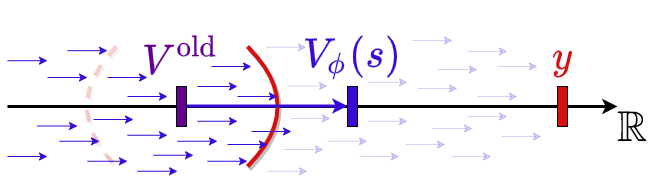
\includegraphics[width=0.4\textwidth]{Images/ValueTrustRegion3.png}
%\vspace{-0.5cm}
\end{wrapfigure}
Наконец, чтобы <<открыть>> trust-region с одной стороны, нужно просто, по аналогии с лоссом актёра, взять максимум от этих двух функций потерь (для актёра мы брали минимум, поскольку там велась максимизация, а здесь лосс минимизируется):
$$\Loss(\phi) \coloneqq \max(\Loss_1(\phi), \Loss_2(\phi))$$
Непосредственной проверкой легко убедиться, что градиенты будут зануляться, только если наш критик вышел из trust-region-а <<с правильной стороны>>; а так, градиенты будут тянуть нашего критика к допустимому барьеру.

\subsection{Proximal Policy Optimizaion (PPO)}

Итоговая процедура работы алгоритма следующая. Собираем большой роллаут (порядка хотя бы 1000 шагов). Версия стратегии, использовавшаяся для сбора, обозначается как $\textcolor{ChadPurple}{\pi^{\old}}$, и вероятности, с которыми она выбирала действия, сохраняются. Для всех пар $s, a$ высчитываются оценки Q-функции и Advatage методом GAE. К собранным данным относимся как к датасету, из которого можно брать пары $s \sim \textcolor{ChadPurple}{d_{\pi^{\old}}}(s), a \sim \textcolor{ChadPurple}{\pi^{\old}}(a \mid s)$ и считать Монте-Карло оценку градиента \eqref{PPOlowerbound}. Размер батча при сэмплировании из датасета при этом обычный для градиентных методов первого порядка, условно такой же, как был бы в A2C. По датасету нужно пройтись при этом несколько раз, теоретически --- сколько угодно, но понятно, что чем больше расходится $\textcolor{ChadBlue}{\pi_\theta}$ и $\textcolor{ChadPurple}{\pi^{\old}}$, тем менее эффективна <<нижняя оценка>> и тем больше данных будет резать наш клиппинг. Количество эпох --- сколько раз пройтись по датасету --- является ключевым гиперпараметром. Существенно, сколько именно шагов градиентного спуска будет сделано по одному датасету; это более важно, чем размер мини-батчей, поскольку именно первое больше влияет на то, когда мы начнём <<вываливаться>> из trust region-а, то есть когда отступим от стратегии сбора данных достаточно далеко. 

\begin{algorithm}[label = PPOalgorithm]{Proximal Policy Optimization (PPO)}
\textbf{Гиперпараметры:} $M$ --- количество параллельных сред, $N$ --- длина роллаутов, $B$ --- размер мини-батчей, $\mathrm{n\_epochs}$ --- количество эпох, $\lambda$ --- параметр GAE-оценки, $\epsilon$ --- параметр обрезки для актёра, $\hat{\epsilon}$ --- параметр обрезки для критика, $V^\pi$ --- нейросеть с параметрами $\phi$, $\pi$ --- нейросеть для стратегии с параметрами $\theta$, $\alpha$ --- коэф. масштабирования лосса критика, SGD оптимизатор.

\vspace{0.3cm}
Инициализировать $\theta, \phi$ \\
\textbf{На каждом шаге:}
\begin{enumerate}
    \item в каждой параллельной среде собрать роллаут длины $N$, используя стратегию $\pi_{\theta}$, сохраняя вероятности выбора действий как $\pi^{\old}(a \mid s)$, а выход критика на встреченных состояниях как $V^{\old}(s) \leftarrow V^{\pi}_{\phi}(s)$
    \item для каждой пары $s, a$ из роллаутов посчитать одношаговую оценку Advantage:
    $$\Psi_{(1)}(s, a) \coloneqq r + \gamma (1 - \done') V^\pi_{\phi}(s') - V^\pi_{\phi}(s)$$
    \item посчитать GAE-оценку:
    $$\Psi_{\mathrm{GAE}}(s_{N-1}, a_{N-1}) \coloneqq \Psi_{(1)}(s_{N-1}, a_{N-1})$$
    \item для $t$ от $N - 2$ до 0:
    \begin{itemize}
    \item $\Psi_{\mathrm{GAE}}(s_t, a_t) \coloneqq \Psi_{(1)}(s_t, a_t) + \gamma \lambda (1 - \done_t) \Psi_{\mathrm{GAE}}(s_{t+1}, a_{t+1})$
    \end{itemize}
    \item посчитать таргет для критика:
    $$y(s) \coloneqq \Psi_{\mathrm{GAE}}(s, a) + V^\pi_{\phi}(s)$$
    \item составить датасет из шестёрок $(s, a, \Psi_{\mathrm{GAE}}(s, a), y(s), \pi^{\old}(a \mid s), V^{\old}(s))$
    \item выполнить $\mathrm{n\_epochs}$ проходов по роллауту, генерируя мини-батчи пятёрок $\T \coloneqq (s, a, \Psi_{\mathrm{GAE}}(s, a), y(s), \pi^{\old}(a \mid s), V^{\old}(s))$ размером $B$; \textbf{для каждого мини-батча:}
    \begin{itemize}
    \item вычислить лосс критика:
    $$\Loss_1(\T, \phi) \coloneqq \left( y(s) - V^\pi_\phi(s) \right) ^2$$
    $$\Loss_2(\T, \phi) \coloneqq \left( y(s) - V^{\old}(s) - \clip(V^\pi_\phi(s) - V^{\old}(s), -\hat{\epsilon}, \hat{\epsilon}) \right) ^2$$
    $$\Loss^{\critic}(\phi) \coloneqq \frac{1}{B}\sum_{\T} \max(\Loss_1(\T, \phi), \Loss_2(\T, \phi))$$
    \item нормализовать $\Psi_{\mathrm{GAE}}(s, a)$ по батчу, чтобы в среднем значения равнялись 0, а дисперсия --- 1.
    \item посчитать коэффициенты в importance sampling:
    $$r_\theta(\T) \coloneqq \frac{\pi_\theta(a \mid s)}{\pi^{\old}(a \mid s)}$$
    \item посчитать обрезанную версию градиентов:
    $$r_\theta^{\clip}(\T) \coloneqq \clip(r_\theta(\T), 1 - \epsilon, 1 + \epsilon)$$
    \item вычислить градиент для актёра:
    $$\nabla^{\actor}_\theta \coloneqq \frac{1}{B}\sum_{\T} \nabla_\theta \min \left( r_\theta(\T)\Psi_{\mathrm{GAE}}(s, a), r_\theta^{\clip}(\T)\Psi_{\mathrm{GAE}}(s, a) \right) $$
    \item сделать шаг градиентного спуска по градиенту $-\nabla^{\actor}_\theta + \alpha \nabla_\phi \Loss^{\critic}(\phi)$
    \end{itemize}
\end{enumerate}
\end{algorithm}

\begin{remark}
PPO использовался для великих достижений в Dota и считается более-менее устоявшейся SOTA в RL (если нет проблем с симулятором и можно использовать on-policy алгоритмы --- стоит начать с PPO), но причины, по которым он так круто работает, полностью не ясны. В частности, \href{https://openreview.net/forum?id=r1etN1rtPB}{последние исследования} указывают на то, что клиппинг --- не основная причина успеха, а кроется она в целом наборе удачных инженерных хаков в официальной реализации алгоритма от OpenAI.
\end{remark}

